\documentclass[conference]{IEEEtran}

\usepackage{cite}
\usepackage{amsmath,amssymb}
\usepackage{graphicx}
\usepackage{booktabs}
\usepackage{array}
\usepackage{url}
\usepackage{balance}
\usepackage[hidelinks]{hyperref}

\graphicspath{{../docs/thesis/figures/chapter4/}}

\title{CAABC-FL: A Hybrid Privacy-Preserving Framework for Secure Multi-Institutional Collaboration}

\hypersetup{
  pdftitle={CAABC-FL: A Hybrid Privacy-Preserving Framework for Secure Multi-Institutional Collaboration},
  pdfauthor={Md. Robiul Islam, Ashrafun Nahar Arifa, Md. Atikur Rahman, Md. Saiful Azad},
  pdfsubject={Privacy-preserving federated learning for multi-institutional healthcare collaboration},
  pdfkeywords={federated learning, healthcare privacy, differential privacy, homomorphic encryption, CKKS, adaptive compression, model poisoning},
  pdfcreator={LaTeX with IEEEtran}
}

\author{
\IEEEauthorblockN{Md. Robiul Islam}
\IEEEauthorblockA{Department of Computer Science\\
and Engineering\\
Green University of Bangladesh\\
Dhaka, Bangladesh\\
{\scriptsize Email: \href{mailto:222002068@student.green.edu.bd}{222002068@student.green.edu.bd}}}
\and
\IEEEauthorblockN{Ashrafun Nahar Arifa}
\IEEEauthorblockA{Department of Computer Science\\
and Engineering\\
Green University of Bangladesh\\
Dhaka, Bangladesh\\
{\scriptsize Email: \href{mailto:222002066@student.green.edu.bd}{222002066@student.green.edu.bd}}}
\and
\IEEEauthorblockN{Md. Atikur Rahman}
\IEEEauthorblockA{Department of Computer Science\\
and Engineering\\
Green University of Bangladesh\\
Dhaka, Bangladesh\\
{\scriptsize Email: \href{mailto:221902166@student.green.edu.bd}{221902166@student.green.edu.bd}}}
\and
\IEEEauthorblockN{Md. Saiful Azad}
\IEEEauthorblockA{Department of Computer Science\\
and Engineering\\
Green University of Bangladesh\\
Dhaka, Bangladesh\\
{\scriptsize Email: \href{mailto:saiful@cse.green.edu.bd}{saiful@cse.green.edu.bd}}}
}

\begin{document}

\maketitle

\begin{abstract}
Cross-silo federated learning enables hospitals to train a shared predictive model without pooling patient records, but local data retention alone does not protect model updates from inference, tampering, poisoning, or communication cost. This paper presents Ciphertext-Aligned Adaptive Block Compression for Federated Learning (CAABC-FL) within a hybrid privacy and trust framework for multi-institutional healthcare learning. The framework combines patient-level differential privacy under add-or-remove-one-patient adjacency, CKKS-based encrypted aggregation, authenticated update submission, independent aggregate verification, validation and rollback controls, threshold-policy model release, and externally witnessed audit checkpoints. CAABC-FL selects a common block support that remains compatible with ciphertext packing and employs error feedback to limit the optimization loss caused by discarded coordinates. The system was evaluated on the 40,336-patient PhysioNet 2019 sepsis cohort while preserving its two natural hospital partitions. Relative to dense DP-FedAvg-CKKS, CAABC-FL reduced the measured serialized encrypted upload by 55.998\%, while the paired AUROC difference was $+0.00017$ (95\% CI: $[-0.00212,+0.00247]$). The AUPRC difference was $-0.00926$, precluding a universal utility-superiority claim. Registered membership-inference attacks remained near chance and differential privacy increased gradient-reconstruction error, but this attack-specific evidence is not proof of privacy. Poisoning experiments further showed that encrypted averaging remains vulnerable without release-time controls; the governance layer contained the evaluated longitudinal backdoor scenario at a measurable utility and availability cost. The results support a bounded utility--communication advantage under the evaluated protocol and clarify the remaining requirements for decentralized key custody, wide-area deployment, and external clinical validation.
\end{abstract}

\begin{IEEEkeywords}
federated learning, healthcare privacy, differential privacy, homomorphic encryption, CKKS, adaptive compression, model poisoning
\end{IEEEkeywords}

\section{Introduction}
\label{sec:introduction}
Clinical prediction models benefit from data that represent different patient
populations, measurement practices, and care pathways. Pooling records from
multiple hospitals can provide this diversity, but it also creates additional
privacy, ownership, consent, and breach risks. Cross-silo federated learning
(FL) offers a different arrangement: hospitals optimize locally and send model
contributions to a coordinating process instead of transferring their source
records. FedAvg established the basic iterative optimization pattern
\cite{mcmahan2017fedavg}, and multi-institutional studies have since demonstrated
its feasibility for medical imaging and outcome prediction
\cite{sheller2020federated,dayan2021federated}.

Keeping records at their originating institutions, however, protects only one
part of the learning pipeline. Model parameters, gradients, and prediction
behaviour can expose information about training examples through membership
inference or reconstruction attacks \cite{shokri2017membership,zhu2019dlg,
geiping2020inverting}. An authenticated participant may also submit a
sign-flipped, replacement, label-flipped, or backdoored update that damages the
shared model \cite{bagdasaryan2020backdoor,fang2020local}. These risks motivate
complementary controls. Differential privacy (DP) limits the influence of a
protected record \cite{dwork2006calibrating,abadi2016deep}; secure aggregation
and homomorphic encryption conceal individual contributions during coordination
\cite{bonawitz2017practical,cheon2017homomorphic}; and authenticated,
auditable services can bind accepted state transitions to identified actors.

These controls have conflicting assumptions. A sparse plaintext vector may
still require dense ciphertexts, while many robust aggregators require the
individual-update geometry that secure aggregation hides. Existing private
compression and robust encrypted systems address parts of this design space
\cite{li2022soteriafl,li2023fedef,asi2025preamble,xu2024ddfed,gu2025dpbrem},
but use different datasets, transport formats, and adversaries.

This paper investigates the resulting integration problem: how can a consortium
protect patient influence and institutional update values, reduce the actual
encrypted traffic, and retain verifiable control over participation,
aggregation, and model release? We present a hybrid research framework and
Ciphertext-Aligned Adaptive Block Compression for Federated Learning
(CAABC-FL). CAABC-FL selects a shared set of contiguous parameter blocks that
maps directly to CKKS ciphertext chunks. Hospitals encrypt only the selected
chunks, while error feedback carries omitted residuals into later rounds. The
common support therefore connects the logical compressor to the serialized
cryptographic representation instead of assuming that a plaintext compression
ratio becomes an equivalent wire reduction.

The framework adds patient-level DP, signed submissions, independent aggregate
recomputation, validation and rollback, and witnessed audit checkpoints. The
evaluation separates the centrally keyed main service from a standalone
multiparty-cryptography experiment and therefore does not claim a fully
decentralized deployment.

The main contributions of this work are as follows:

\begin{itemize}
    \item We design and implement an end-to-end cross-silo framework that
    combines patient-level DP, CKKS aggregation, authenticated submissions,
    independent aggregate verification, validation and rollback, controlled
    release, and witnessed auditing under one explicit threat model.

    \item We introduce CAABC-FL, which co-designs adaptive shared-block
    selection, CKKS packing, and error feedback so that compression is measured
    from serialized encrypted uploads rather than inferred from retained
    plaintext coordinates.

    \item We conduct a paired, multi-seed evaluation on the full 40,336-patient
    PhysioNet 2019 sepsis cohort \cite{reyna2020early,physionet2019sepsis}. The
    study compares optimization, private, encrypted, compressed, and
    same-protocol SOTA-style baselines under benign and adversarial conditions,
    including membership inference, gradient reconstruction, one-round and
    longitudinal poisoning, cryptographic correctness, failure recovery, and
    service overhead.
\end{itemize}

Against dense DP-FedAvg-CKKS, CAABC-FL reduced serialized upload by $55.998\%$
and passed the registered AUROC non-inferiority gate. Its AUPRC difference was
$-0.00926$, preventing a universal superiority claim. Privacy attacks were near
chance for the evaluated DP methods, whereas encrypted mean remained vulnerable
to poisoning; governed release contained the tested longitudinal backdoor at
utility and availability cost.

\section{Related Work}
\label{sec:related-work}

\subsection{Healthcare Federated Learning}

Early medical FL studies primarily examined whether collaboration across natural
institutional boundaries could retain useful predictive performance. Sheller
\emph{et al.} trained brain-tumour segmentation models across ten institutions,
while Dayan \emph{et al.} developed the EXAM COVID-19 outcome model using data
from twenty institutions \cite{sheller2020federated,dayan2021federated}. These
studies provide important evidence that distributed clinical learning is
feasible, but privacy attacks, encrypted transport, poisoning, and release
governance were not evaluated as one system. FLamby later improved
reproducibility by providing seven healthcare datasets with natural silo
partitions and standardized baselines \cite{ogier2022flamby}. OpenFL similarly
supports practical medical FL experiments and deployments
\cite{foley2022openfl}. Together, this literature motivates evaluation on real
institutional partitions rather than randomly assigning a small pooled table to
simulated clients.

FedProx, SCAFFOLD, and FedNova address heterogeneous objectives, client drift,
or unequal local work \cite{li2020fedprox,karimireddy2020scaffold,wang2020fednova},
but do not independently provide privacy or poisoning resistance.

\subsection{Differential Privacy and Protected Aggregation}

DP and cryptography protect different parts of FL. DP bounds the influence of a
protected training unit on the released output
\cite{dwork2006calibrating,abadi2016deep}, whereas secure aggregation or
homomorphic encryption restricts what the coordinator can observe during
training \cite{bonawitz2017practical,cheon2017homomorphic}. Privacy-first health
studies have demonstrated DP-enabled federated analysis across several clinical
modalities \cite{sadilek2021privacy}. FAMHE further showed that multiparty HE can
support biomedical survival and genomic analyses without assigning decryption
to one central party \cite{froelicher2021famh}. POSEIDON demonstrated encrypted
collaborative neural-network training, although its passive-adversary and
non-clinical evaluation differs from active cross-silo healthcare threats
\cite{sav2021poseidon}.

FLDP combines distributed DP noise with malicious-secure private aggregation
\cite{stevens2022fldp}, but does not include a poisoning layer. Near-chance
empirical attacks are not formal DP guarantees, and encryption alone does not
limit what a released model reveals.

\subsection{Communication Efficiency Under Encryption}

Most FL compressors measure retained coordinates or idealized bits before
encryption. Fed-EF analyzes biased compression and error feedback under non-IID
data, while SoteriaFL studies privacy and shifted compression jointly
\cite{li2023fedef,li2022soteriafl}. These methods establish important
optimization and privacy relationships, but a client-specific sparse vector may
still require dense CKKS encoding when its support must remain hidden. Thus,
logical sparsity does not necessarily imply an encrypted-wire reduction.

PREAMBLE co-designs block-sparse vectors with a two-server private aggregation
protocol \cite{asi2025preamble}. CAABC-FL instead uses common adaptive blocks,
CKKS chunks, and error feedback in iterative healthcare training, making
PREAMBLE an architectural rather than directly interchangeable comparator.

\subsection{Poisoning Resistance and Governance}

Krum, coordinate median, trimmed mean, and robust federated aggregation replace
ordinary averaging with distance-, coordinate-, or geometric-median rules
\cite{blanchard2017krum,yin2018byzantine,pillutla2022robust}. FLTrust instead
uses a trusted root update to score client directions \cite{cao2021fltrust}.
These defences are effective under their stated attacker and visibility
assumptions, but they normally inspect individual plaintext updates. A sum-only
encrypted coordinator cannot apply them directly without additional secure
computation or disclosure.

DDFed uses encrypted anomaly detection \cite{xu2024ddfed}, while DP-BREM+
combines secure aggregation, jointly generated DP noise, history, and momentum
\cite{gu2025dpbrem}. Neither evaluates CKKS-aligned adaptive compression,
independent aggregate verification, and witnessed release on the target cohort.
Permissioned ledgers provide authenticated policy validation
\cite{androulaki2018hyperledger}, but a recorded hash alone does not prove
correct aggregation.

\subsection{Synthesis and Research Gap}

Three gaps remain: protection mechanisms are usually evaluated in separate
protocols; logical compression is often reported without serialized encrypted
cost; and protected aggregation hides the geometry required by many robust
rules. CAABC-FL addresses the second gap through common ciphertext-aligned
blocks, while the framework evaluates verification, rollback, and witnessed
auditing under one protocol. It does not claim universal poisoning resistance or
full decentralization.

\section{Threat Model and Design Goals}
\label{sec:threat-model}

\subsection{System Roles and Protected Assets}

The consortium contains $K$ authenticated healthcare institutions, a coordinating
service, a decryption authority, an independent aggregate verifier, audit
witnesses, and authorized inference users. Each hospital retains its patient
records and signing key, trains from an approved global-model version, and
submits a signed encrypted update. The coordinator admits protocol-compatible
messages and computes a weighted CKKS sum, but has no CKKS secret key. The
authority verifies a decryption request and releases only an approved aggregate.
The verifier independently reconstructs the accepted transcript and aggregate
evidence. Three separately keyed witnesses persist ordered checkpoints; the
implemented policy requires two signed receipts.

The protected assets are: (i) patient records and features; (ii) individual
hospital updates and local statistics; (iii) signing and decryption keys; (iv)
the integrity and version history of the global model; (v) participation,
privacy, and release metadata; and (vi) the continuity of the audit record. Raw
patient data, identifiers, and row-level measurements are not transferred to the
coordinator.

\subsection{Adversary Capabilities}

Hospitals are identifiable consortium members, but a subset may be Byzantine.
They may submit malformed, scaled, sign-flipped, model-replacement, ALIE,
label-flipped, backdoored, colluding, sleeper, or adaptively timed updates. A
Sybil attempt is considered at the admission boundary, where each accepted
identity must possess a registered credential. No fixed Byzantine fraction is
assumed as a universal guarantee; attacker participation is varied explicitly in
the experiments.

For confidentiality analysis, the coordinator is honest-but-curious: it follows
the aggregation interface while attempting to infer information from the
ciphertexts, metadata, and released models. The integrity tests additionally
allow it to omit, replay, reorder, or replace an accepted contribution and to
present a forged aggregate for decryption. External network adversaries may
eavesdrop, tamper, replay, or impersonate a service. Model-level adversaries may
perform membership inference or gradient reconstruction using only the
information assigned by the registered attack protocol
\cite{shokri2017membership,zhu2019dlg,geiping2020inverting}.

The two-of-three witness policy tolerates one outage but not coordinator-plus-two-
witness collusion. Validation and reputation are empirical release controls; a
stealthy attacker may remain within the acceptance threshold.

\subsection{Trust Assumptions and Exclusions}

The main TenSEAL service treats the authority as a trusted plaintext boundary
because it owns one CKKS secret key. The authority is policy constrained: it
rechecks hospital envelopes, round and model-version binding, participant
manifest, nonce state, and the aggregate digest before decryption. A separate
three-of-three OpenFHE experiment demonstrates multiparty decryption, but it is
not integrated into the main service and is not claimed as dropout-tolerant
networked key custody. Hospitals are trusted to protect their local host and
long-term signing keys; they are not trusted to submit an honest learning update.

The model excludes physical compromise of hospital hardware, side-channel or
cryptanalytic attacks against the selected libraries, compromise of the central
authority, compromise of a majority witness quorum, and formal verification of
the custom random-number path. It also excludes a real wide-area hospital
deployment, hardware-attested TDX/SNP execution, prospective clinical safety,
and regulatory certification. These boundaries prevent the prototype evidence
from being described as a fully decentralized or production-approved system.

\subsection{Design Goals}

The design goals are to: (i) bound one patient's influence through recorded DP;
(ii) hide individual hospital updates; (iii) authenticate and bind every message
to its identity, round, version, support, nonce, and digest; (iv) reduce
serialized CKKS bytes while retaining utility; (v) verify and validate a
candidate before release; and (vi) preserve independently checkable evidence and
recover after a bounded outage. Section~\ref{sec:limitations} maps these controls
to residual risks.

\section{Proposed Framework}
\label{sec:framework}

\subsection{End-to-End Round Architecture}

Hospital $k$ retains $\mathcal{D}_k$, preprocessing state, a signing key, CAABC
residual, and the public CKKS context. The coordinator owns no secret key. The
authority controls main-service decryption, the verifier reconstructs accepted
aggregation evidence, and witnesses store signed checkpoint hashes.

At round $t$, hospitals accept only a signed global model $\theta_t$ whose
version and digest match the announced round. Each hospital trains locally,
applies patient-level DP, projects the private update onto a shared
ciphertext-aligned support, encrypts the packed values, and signs the complete
message envelope. The coordinator rejects invalid or stale envelopes before
homomorphic aggregation. The authority decrypts only after independent
aggregate verification. A candidate is then evaluated on disjoint validation
data and is either committed or rolled back. Table~\ref{tab:round-protocol}
summarizes this sequence.

\begin{table*}[t]
\caption{Authenticated and governed CAABC-FL round}
\label{tab:round-protocol}
\centering
\scriptsize
\setlength{\tabcolsep}{4pt}
\renewcommand{\arraystretch}{1.1}
\begin{tabular}{@{}p{0.7cm}p{2.8cm}p{7.0cm}p{5.3cm}@{}}
\toprule
Step & Role & Operation & Enforced evidence or decision \\
\midrule
1 & Coordinator & Broadcast signed $\theta_t$, model digest, round, protocol identifier, and current support policy & Hospitals reject an invalid signature, stale version, or incompatible protocol \\
2 & Hospital & Train locally; clip per-patient gradients; add calibrated noise; update the privacy accountant & Raw records remain local; privacy metadata is bound to the submission \\
3 & Hospitals/authority & On a refresh round, encrypt and aggregate DP-derived block scores; release only their verified aggregate & Common support $S_t$ is selected without exposing client-specific supports \\
4 & Hospital & Add error-feedback residual, project onto $S_t$, CKKS-encrypt, hash, and sign the update envelope & Identity, version, round, nonce, timestamp, support, record count, and ciphertext digest are bound \\
5 & Coordinator & Admit valid envelopes and compute the record- and reputation-weighted encrypted sum & Replays, stale messages, unknown identities, and support/context mismatches are rejected \\
6 & Verifier/authority & Re-verify original envelopes, independently recompute the encrypted aggregate, compare digests, and decrypt only a match & Omission, substitution, or inconsistent weighting causes rejection \\
7 & Validators & Evaluate the candidate on disjoint validation data and sign accept/reject decisions & Accepted candidate is committed; otherwise $\theta_t$ remains active \\
8 & Witnesses & Sign the ordered round checkpoint and persist model, decision, and transcript digests & Two receipts establish the implemented checkpoint quorum and support restart reconciliation \\
\bottomrule
\end{tabular}
\end{table*}

\subsection{Private Local Update}

Per-patient gradients are clipped at norm $C$, averaged with Gaussian noise
$\mathcal{N}(0,\sigma^2C^2I)$, and composed with the recorded accountant to
produce $\widetilde{\Delta}_{k,t}$ following DP-SGD \cite{abadi2016deep}. CAABC
observes only this sanitized update, so scoring, support selection, packing, and
encryption are post-processing rather than new accesses to unclipped gradients.

\subsection{Ciphertext-Aligned Adaptive Block Compression}

Let $d$ be the number of model parameters and let $r_{k,t}\in\mathbb{R}^d$ be
hospital $k$'s residual. CAABC first forms
\begin{equation}
u_{k,t}=\widetilde{\Delta}_{k,t}+r_{k,t}.
\label{eq:paper-effective-update}
\end{equation}
The coordinates are partitioned into $q=\lceil d/B\rceil$ contiguous blocks
$I_1,\ldots,I_q$ of at most $B$ values. On a support-refresh round, hospital
$k$ computes a DP-derived block score
\begin{equation}
s_{k,t,b}=\left\lVert\widetilde{\Delta}_{k,t}[I_b]\right\rVert_2.
\label{eq:paper-block-score}
\end{equation}
Score vectors are encrypted and combined before release. Using record weights
$\alpha_k=n_k/\sum_j n_j$, the common support is
\begin{equation}
S_t=\arg\max_{S\subseteq\{1,\ldots,q\}}
\sum_{b\in S}\sum_k\alpha_k s_{k,t,b}
\quad\text{s.t.}\quad
\sum_{b\in S}|I_b|\leq cL,
\label{eq:paper-caabc-support}
\end{equation}
where $L$ is the CKKS slot capacity and $c$ is the update-ciphertext budget.
All hospitals therefore pack the same coordinates in the same order. This avoids
revealing a client-specific Top-$k$ support and, unlike dense re-encoding,
allows logical block selection to reduce the number of transmitted ciphertexts.

Let $P_{S_t}$ pack the selected blocks and $P_{S_t}^{\mathsf T}$ scatter them
back into the dense layout. The transmitted vector and next residual are
\begin{equation}
p_{k,t}=P_{S_t}(u_{k,t}),\qquad
r_{k,t+1}=u_{k,t}-P_{S_t}^{\mathsf T}p_{k,t}.
\label{eq:paper-error-feedback}
\end{equation}
Thus, omitted information is retained locally rather than permanently discarded.
The frozen configuration uses $d=18{,}049$, $B=256$, $L=4096$, $c=2$, and a
support refresh every $R=5$ rounds. A dense update requires five CKKS chunks,
whereas CAABC targets two update chunks and amortizes one encrypted score vector
over the refresh interval. Serialized byte counts, rather than this analytical
chunk count, determine the reported communication result.

\subsection{Authenticated Encrypted Aggregation}

Hospital $k$ encrypts $p_{k,t}$ and signs an envelope containing its identity,
round, source-model version, privacy metadata, record count, support identifier,
timestamp, nonce, CKKS-context identifier, and ciphertext digest. An envelope is
admissible only when all bindings and the signature are valid and the nonce is
unused. For the admitted set $\mathcal{K}_t^+$, the coordinator computes
\begin{equation}
C_t=\sum_{k\in\mathcal{K}_t^+}\beta_{k,t}
\operatorname{Enc}_{pk}(p_{k,t}),\qquad
\beta_{k,t}=\frac{n_k\rho_{k,t}}
{\sum_{j\in\mathcal{K}_t^+}n_j\rho_{j,t}},
\label{eq:paper-encrypted-aggregate}
\end{equation}
where $\rho_{k,t}$ is the current reputation multiplier. CKKS permits the
required approximate additions and plaintext-scalar multiplications without
decrypting an individual update \cite{cheon2017homomorphic}.

The authority rechecks the original envelopes, reconstructs
Eq.~\eqref{eq:paper-encrypted-aggregate}, and permits decryption only if the
participant quorum is met, the request is fresh, and
\begin{equation}
H(C_t^{\mathrm{verifier}})=H(C_t^{\mathrm{coordinator}}).
\label{eq:paper-aggregate-verification}
\end{equation}
This detects tested omission, substitution, and inconsistent weighting but is
not a zero-knowledge proof. Only the aggregate update
$\widehat{\Delta}_t=P_{S_t}^{\mathsf T}\operatorname{Dec}(C_t)$ is released to
form candidate $\theta'_t=\theta_t+\widehat{\Delta}_t$.

\subsection{Governed Release and Audit Evidence}

Validator $v$ accepts the candidate when its loss on a disjoint validation
partition does not exceed the previous-model loss by more than tolerance $\tau$:
\begin{equation}
a_{v,t}=\mathbb{I}\!\left[
L_v(\theta'_t)\leq L_v(\theta_t)+\tau\right].
\label{eq:paper-validation}
\end{equation}
If the required signed-vote fraction is reached, $\theta'_t$ is atomically
committed as $\theta_{t+1}$; otherwise the service rolls back to $\theta_t$.
Rejections update reputation and may quarantine a participant, but validation
does not prove that every committed model is free of a stealthy backdoor.

Each event extends hash chain $h_t=H(h_{t-1}\Vert e_t)$ and requires signatures
from two of three witnesses. Events contain digests and decisions rather than
private updates. The policy tolerates one outage but is not blockchain or BFT
consensus.

\section{Experimental Methodology}
\label{sec:methodology}

\subsection{Dataset, Split, and Preprocessing}

The primary dataset is the 2019 PhysioNet/Computing in Cardiology Challenge
sepsis cohort
\cite{reyna2020early,physionet2019sepsis}. The released training data contain
40,336 patients from two natural source partitions: Hospital A contains 20,336
patients with 1,790 positive cases, and Hospital B contains 20,000 patients with
1,142 positive cases. The resulting overall prevalence is 7.27\%. Preserving
these sources provides a natural cross-silo evaluation rather than an artificial
random client partition.

Within each hospital, patients are stratified and split 70/15/15 into training,
validation, and locked test sets. A positive patient's landmark is the first
positive hour; a control landmark is drawn deterministically from the
training-case landmark distribution. Seven summaries of each of 40 variables
over the preceding 24 hours produce 280 features. Standardization and class
weights use training patients only. This pooled preprocessing ran on the
research host and is not claimed as a secure federated-analytics service.

\subsection{Frozen Training and Cryptographic Configuration}

The classifier is a 280--64--1 multilayer perceptron with ReLU activation and
18,049 trainable parameters. Every paired method uses the same patient split,
initialization seed, 20-round budget, one local epoch per round, batch size 128,
and learning rate 0.03. The operating threshold maximizes Youden's $J$ on pooled
validation predictions for each method and seed and is then frozen for all test
reporting.

The private methods use per-patient clipping $C=1.0$, Gaussian noise multiplier
$\sigma=1.2$, $\delta=10^{-5}$, Poisson sampling, and an RDP accountant. CKKS is
implemented with TenSEAL 0.3.17 using polynomial modulus degree 8192,
coefficient-modulus bits $(60,40,40,60)$, and scale $2^{40}$. CAABC uses
256-coordinate blocks, two update-ciphertext chunks, a five-round support-refresh
interval, and error feedback. These values and all decision rules were frozen
before confirmatory test access.

\subsection{Baselines and Experimental Matrix}

The utility tier includes FedAvg, FedProx, SCAFFOLD, FedNova, FedAdam, and
FedYogi, together with local-only and centralized references. The core protected
tier contains DP-FedAvg, dense DP-FedAvg-CKKS, CAABC-static, and CAABC-FL over ten
paired seeds. Five-seed secondary controls include Random-$k$, client Top-$k$,
error-feedback Top-$k$, fixed public blocks, and quantized updates. Client-specific
supports and quantization metadata are re-encoded into dense CKKS when required
to conceal them; these methods receive no encrypted-wire-saving credit merely
for reducing a plaintext representation.

Fed-EF-SGD, Fed-EF-AMS, and SoteriaFL-SGD are additionally adapted over five
paired seeds to the same cohort, model, patient-level DP, round budget, and CKKS
backend \cite{li2023fedef,li2022soteriafl}. They are same-protocol comparisons,
not reproductions of the papers' original dataset values.

\subsection{Privacy, Poisoning, and Service Tests}

The powered membership experiment uses 720 members and 720 label-matched
non-members per seed. Online LiRA and RMIA use eight architecture-matched
reference models per seed and report attack AUC, advantage, and low-FPR TPR
\cite{carlini2022membership}. Gradient reconstruction runs for 300 optimization
steps on four records per seed under exact plaintext, CAABC-masked,
DP-sanitized, and combined DP--CAABC observations
\cite{zhu2019dlg,geiping2020inverting}.

The poisoning matrix uses 20 virtual clients, seven attacks, six aggregation
rules, malicious fractions 0.1--0.4, and five-/twenty-round adaptive extensions.
Coordinate median, trimmed mean, Multi-Krum, geometric median, and FLTrust are
assumption-mismatched diagnostics requiring plaintext geometry or a trusted root
\cite{blanchard2017krum,yin2018byzantine,pillutla2022robust,cao2021fltrust}.
Only weighted encrypted aggregation followed by global validation is directly
compatible with the implemented sum-only CKKS service.

Full-cohort training and attacks run in the scientific profile. A containerized
service profile separately tests authentication, persistence, verification,
rollback, and witness recovery on controlled vectors; its latency is not a WAN
production benchmark.

\subsection{Outcomes and Statistical Analysis}

Predictive outcomes include accuracy, precision, sensitivity, specificity, F1,
balanced accuracy, Matthews correlation coefficient, AUROC, AUPRC, Brier score,
and calibration parameters. AUROC and AUPRC are emphasized because the endpoint
is imbalanced. Privacy outcomes include the final $(\epsilon,\delta)$ budget,
membership-attack measures, and reconstruction RMSE. Poisoning outcomes are
computed relative to a clean run of the same seed and defence and include
utility change, backdoor attack-success-rate (ASR) change, rollback, quarantine,
and clean-utility cost.

Communication is measured from serialized ciphertext objects. If
$B_{\mathrm{packed}}$ is the packed update upload, $B_{\mathrm{scores}}$ is the
amortized encrypted score traffic, and $B_{\mathrm{dense}}$ is the dense
DP-FedAvg-CKKS upload, then
\begin{equation}
R_{\mathrm{wire}}=1-
\frac{B_{\mathrm{packed}}+B_{\mathrm{scores}}}{B_{\mathrm{dense}}}.
\label{eq:paper-wire-reduction}
\end{equation}
This value is reported separately from logical coordinate reduction.
Encryption, signing, verification, aggregation, recomputation, decryption,
audit, and end-to-end latency are recorded when exposed by the execution path.

The model seed is the statistical unit; patients, virtual clients, and attack
trials from one trained model are not treated as independent replicates. For
paired seed-level differences $d_s$, two-sided Student-$t$ 95\% confidence
intervals are
\begin{equation}
\bar d\ \pm\ t_{0.975,n-1}\frac{s_d}{\sqrt{n}}.
\label{eq:paper-paired-ci}
\end{equation}
The confirmatory claim requires both the lower confidence bound of the paired
CAABC-minus-dense AUROC difference to exceed $-0.015$ and the lower confidence
bound of $R_{\mathrm{wire}}$ to exceed 0.40. Secondary outcomes remain
exploratory. Holm adjustment is applied within registered privacy, poisoning,
longitudinal, and ablation endpoint families.

Reproducibility controls include frozen JSON protocols, raw and processed data
hashes, patient-split digests, a first-test-access marker, resumable experiment
cells, schema validation, output hashes, environment manifests, and
prediction-level exports. Because CKKS encryption and secure noise are
randomized, replication targets numerical tolerances, serialized-size
distributions, and aggregate statistics rather than byte-identical ciphertexts.

\section{Results and Discussion}
\label{sec:results}

\subsection{Predictive Utility and Encrypted Communication}

Table~\ref{tab:paper-core-results} reports the ten-seed core comparison. The
non-private FedAvg reference reached AUROC 0.830 and AUPRC 0.471. DP-FedAvg and
dense DP-FedAvg-CKKS both reached AUROC near 0.73 and AUPRC 0.394, indicating
that most of the observed utility reduction was associated with clipping and
noise rather than CKKS approximation. The protected methods used the recorded
budget $(\epsilon,\delta)=(1.935,10^{-5})$.

\begin{table}[t]
\caption{Core test performance and encrypted upload}
\label{tab:paper-core-results}
\centering
\scriptsize
\setlength{\tabcolsep}{2.7pt}
\begin{tabular}{@{}lccccc@{}}
\toprule
Method & AUROC & AUPRC & Sens. & F1 & MB/round \\
\midrule
FedAvg & .830 & .471 & .757 & .292 & -- \\
DP-FedAvg & .732 & .394 & .458 & .293 & -- \\
DP-FedAvg-CKKS & .731 & .394 & .457 & .296 & 3.314 \\
CAABC-static & .732 & .390 & .476 & .282 & 1.359 \\
CAABC-FL & .731 & .384 & .534 & .253 & 1.458 \\
\bottomrule
\end{tabular}
\end{table}

CAABC-FL changed the operating point despite retaining the dense reference's
AUROC: sensitivity increased from 0.457 to 0.534, while specificity decreased
from 0.862 to 0.776 and F1 decreased from 0.296 to 0.253. Thus, accuracy or AUROC
alone would conceal clinically relevant trade-offs. Communication behaved more
decisively. CAABC-FL reduced mean serialized encrypted upload from 3.314 to
1.458 MB per round. In contrast, client-specific Top-$k$, error-feedback Top-$k$,
and quantization required dense CKKS re-encoding to protect their metadata and
therefore produced no measured wire reduction.

The two pre-specified decision gates are shown in
Table~\ref{tab:paper-confirmatory-gates}. The paired CAABC-minus-dense AUROC
difference was $+0.00017$ with a 95\% CI of
$[-0.00212,+0.00247]$, whose lower bound exceeded the $-0.015$
non-inferiority margin. Mean encrypted-wire reduction was $55.998\%$ with a
95\% CI of $[55.994\%,56.002\%]$, exceeding the 40\% target. Both primary gates
therefore passed. However, the AUPRC difference was $-0.00926$ and its entire
interval was negative; Brier score also increased by 0.00211
$[0.00177,0.00245]$. The supported claim is an AUROC-preserving encrypted-
communication trade-off, not superiority on every predictive measure.

\begin{table}[t]
\caption{CAABC-FL decision gates versus dense DP-FedAvg-CKKS}
\label{tab:paper-confirmatory-gates}
\centering
\scriptsize
\setlength{\tabcolsep}{3pt}
\begin{tabular}{@{}lccc@{}}
\toprule
Endpoint & Effect (95\% CI) & Rule & Result \\
\midrule
AUROC difference & $+.00017$ [$-.00212,+.00247$] & LCB $>-.015$ & Pass \\
Wire reduction & 55.998\% [55.994\%,56.002\%] & LCB $>40\%$ & Pass \\
AUPRC difference & $-.00926$ [$-.01160,-.00691$] & Descriptive & Adverse \\
\bottomrule
\end{tabular}
\end{table}

In the five-seed same-protocol comparison
(Fig.~\ref{fig:paper-sota-tradeoff}), all private methods reached AUROC
0.727--0.732. CAABC-FL obtained 0.730 $[0.727,0.734]$ and 56\% wire reduction;
Fed-EF and SoteriaFL variants had overlapping utility but no saving after dense
CKKS transport. Eight post-hoc locked non-inferiority tests passed after Holm
adjustment, but mixed AUPRC effects preclude superiority.

\begin{figure}[t]
\centering
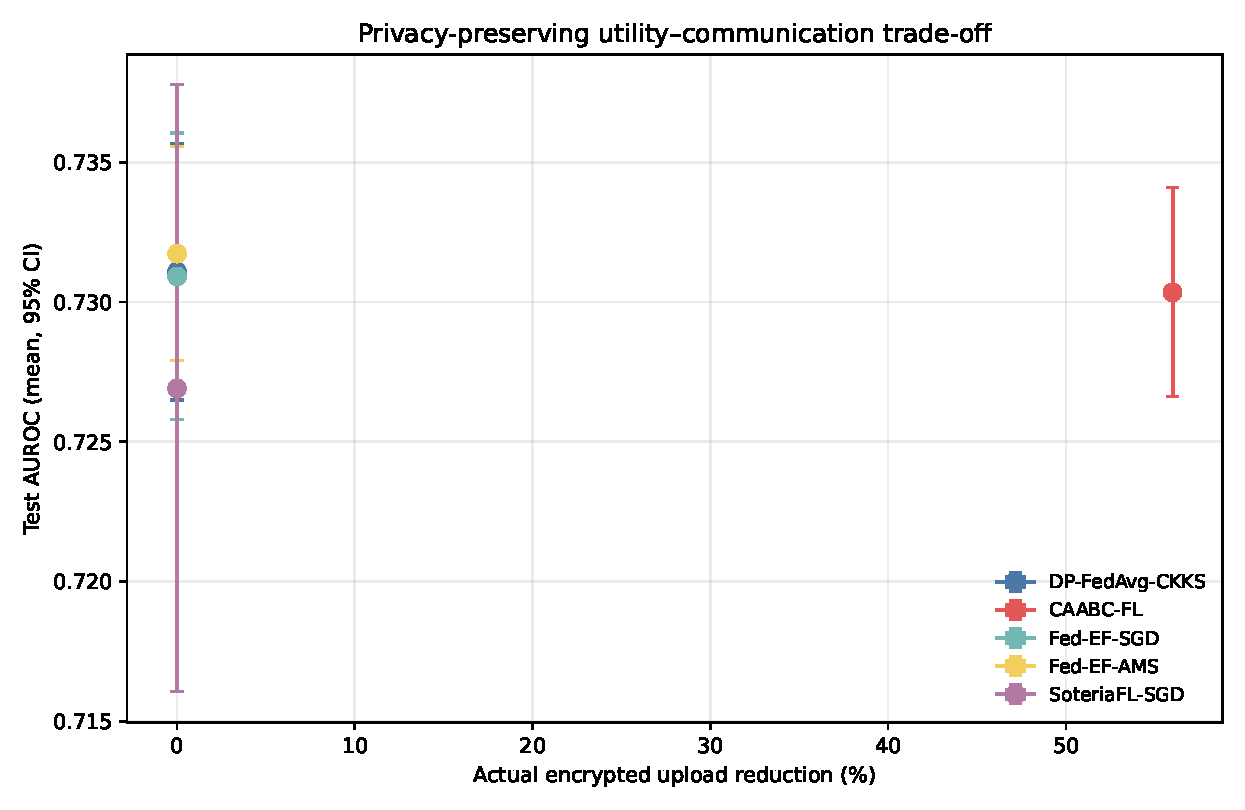
\includegraphics[width=\columnwidth]{sota_utility_wire_tradeoff.pdf}
\caption{Same-protocol utility and measured encrypted-upload trade-off over five paired seeds.}
\label{fig:paper-sota-tradeoff}
\end{figure}

\subsection{Privacy-Attack Evidence}

The powered membership attack produced AUROC 0.5239
$[0.5085,0.5393]$ for FedAvg, 0.5050 $[0.4922,0.5179]$ for dense
DP-FedAvg-CKKS, and 0.5035 $[0.4929,0.5142]$ for CAABC-FL. The paired
CAABC-minus-FedAvg difference was $-0.0204$ $[-0.0457,+0.0050]$; because the
interval crosses zero, the experiment does not establish direct privacy
superiority.

In Fig.~\ref{fig:paper-security-results}, RMIA reached 0.5492
$[0.5220,0.5763]$ for FedAvg but 0.5067 and 0.5063 for dense DP-CKKS and
CAABC-FL; online LiRA gave CAABC-FL 0.4963. These attack-specific outcomes do
not replace the privacy accountant.

Gradient reconstruction showed a clearer separation. After 300 optimization
steps, plaintext-exact observations yielded mean feature RMSE 0.684, compared
with 2.547 for DP-sanitized observations and 2.763 for the worst-case combined
DP--CAABC exposure. The paired increase from plaintext to DP--CAABC was 2.079
$[1.844,2.313]$. Compression alone did not provide comparable protection, so the
result should be attributed primarily to DP and to the assumed observation path,
not to CAABC as an independent privacy mechanism.

\subsection{Poisoning and Governed Release}

The right panel of Fig.~\ref{fig:paper-security-results} summarizes the most
severe one-round setting. With 40\% malicious clients, ordinary weighted mean
lost 0.393 AUROC $[-0.421,-0.366]$ under model replacement and backdoor ASR
increased by 0.888. FLTrust and Multi-Krum controlled these attacks more
consistently, but require a trusted root update or individual plaintext geometry
and are therefore not deployable inside the implemented sum-only CKKS path.
This confirms that encryption and compression are not poisoning defences.

\begin{figure*}[t]
\centering
\begin{minipage}{0.49\textwidth}
\centering
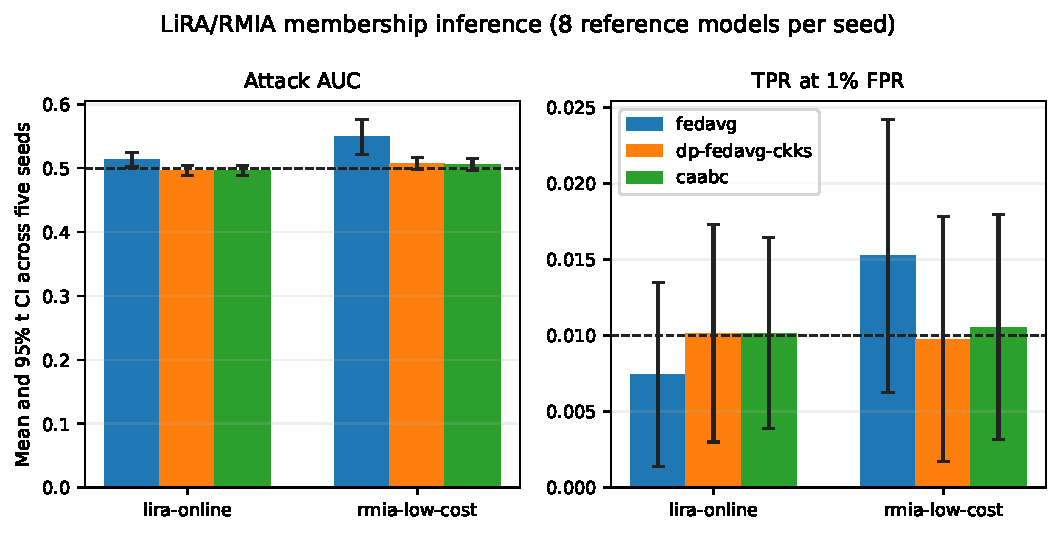
\includegraphics[width=\linewidth]{advanced_privacy.pdf}\\[-1mm]
\footnotesize (a) LiRA/RMIA membership-inference diagnostics.
\end{minipage}\hfill
\begin{minipage}{0.49\textwidth}
\centering
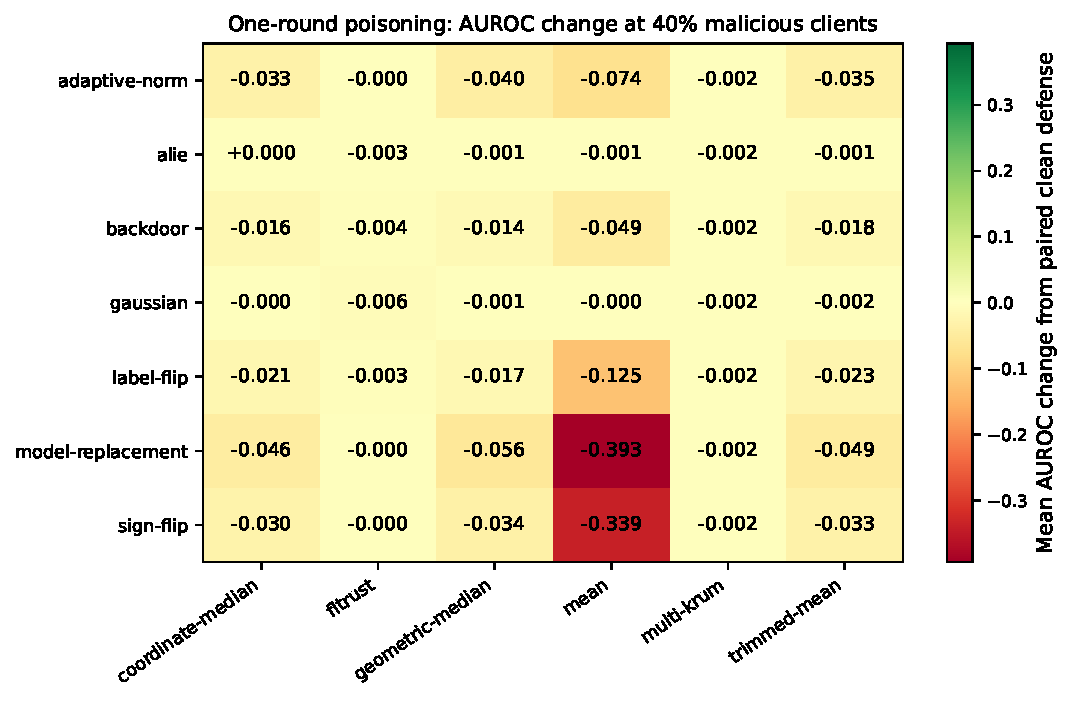
\includegraphics[width=\linewidth]{poisoning_heatmap.pdf}\\[-1mm]
\footnotesize (b) One-round AUROC change at 40\% malicious clients.
\end{minipage}
\caption{Five-seed privacy and poisoning evidence. Membership AUROC near 0.5 indicates chance-level discrimination by the registered attacks; poisoning cells report mean paired AUROC changes from clean training.}
\label{fig:paper-security-results}
\end{figure*}

At 40\% malicious clients, the longitudinal backdoor ended with ASR change
$+0.0046$ $[-0.0501,+0.0592]$; all malicious clients were quarantined and 60\%
of rounds rolled back, but clean AUROC fell 0.0293 $[-0.0413,-0.0173]$.
Replacement and sign flip remained more variable. The gate therefore contained
the evaluated backdoor at utility and availability cost, not with a formal
Byzantine guarantee.

\subsection{Systems, Governance, and Ablation Findings}

Service tests rejected invalid, stale, replayed, unauthorized, and forged
requests. Two witness receipts tolerated one outage and supported restart
reconciliation. Isolated OpenFHE 3-of-3 CKKS achieved maximum error
$1.34\times10^{-13}$ and failed without one share, demonstrating multiparty
functionality but not an integrated dropout-tolerant threshold service.

The single-host mTLS/CKKS service scaled from 1.337 s for two clients to 7.080 s
for sixteen clients, while encrypted upload increased from 3.16 to 25.28 MiB.
The near-linear descriptive fit cannot be generalized to WAN or concurrent
multi-host execution. The CAABC ablation showed the expected frontier: one chunk
increased wire reduction to about 76\% but increased utility variation; refreshing
support every round reduced the saving to about 40\%, whereas a ten-round refresh
increased it to about 58\%. Removing error feedback changed mean AUROC by
approximately $-0.0010$ with an interval crossing zero. The selected two-chunk,
five-round-refresh configuration is therefore a registered compromise rather
than an optimum for every outcome.

\subsection{Overall Interpretation}

Three conclusions follow. First, DP, encryption, compression, and robustness
must be evaluated jointly: privacy can remove update visibility, dense encrypted
encoding can erase logical compression, and rollback can trade availability for
integrity. Second, the strongest measured improvement is specific and
reproducible: CAABC-FL converted common adaptive blocks into approximately 56\%
less serialized CKKS traffic while meeting the AUROC non-inferiority gate.
Third, the negative findings are essential to the claim boundary. AUPRC and
several operating-point metrics declined; empirical attacks cannot prove
privacy; encrypted mean remained poisonable; and witnessed auditing did not
remove the central authority. The framework is consequently supported as an
integrated research system and communication--utility trade-off, not as a
universally superior, poisoning-proof, or fully decentralized clinical platform.

\section{Security Analysis and Limitations}
\label{sec:limitations}

\subsection{Security Properties and Residual Risk}

The framework provides layered protection, not one composite proof. Patient-level
DP applies under its declared adjacency, sampling, clipping, noise, and
accountant assumptions; CAABC operates as post-processing. Membership and
reconstruction tests remain attack-specific diagnostics.

CKKS hides individual values from the honest-but-curious coordinator, while
mutual authentication, signatures, and version/nonce bindings protect message
integrity. Identities, timing, sizes, common support, and accepted weights remain
visible; endpoint compromise and side channels are excluded.

Independent recomputation detects tested omission, substitution, and inconsistent
weighting, but is not a zero-knowledge proof and does not verify honest local
training. Witness checkpoints are tamper-evident evidence, not Byzantine
consensus.

Validation is compatible with sum-only CKKS but may miss stealthy attacks,
reject useful distribution shifts, or enable rollback-based denial of service.
Table~\ref{tab:paper-security-boundaries} separates evidence from assumptions.

\begin{table*}[t]
\caption{Demonstrated security evidence and claim boundaries}
\label{tab:paper-security-boundaries}
\centering
\scriptsize
\setlength{\tabcolsep}{4pt}
\renewcommand{\arraystretch}{1.1}
\begin{tabular}{@{}p{2.7cm}p{5.3cm}p{4.1cm}p{4.4cm}@{}}
\toprule
Property & Implemented evidence & Supported interpretation & Unsupported extension \\
\midrule
Patient privacy & Recorded $(\epsilon,\delta)$ accountant; loss, LiRA/RMIA, and reconstruction tests & Formal DP under stated mechanism plus attack-specific empirical evidence & Proof that membership or reconstruction is impossible \\
Update confidentiality & Real CKKS ciphertexts; coordinator has public context only & Individual values hidden from the honest-but-curious coordinator in the intended path & Protection after endpoint/key compromise or against implementation side channels \\
Message integrity & Signed envelopes; mTLS; identity, digest, version, nonce, timestamp, and replay checks & Invalid, stale, modified, and replayed tested messages are rejected & Compromised hospital credentials imply an honest update \\
Aggregate integrity & Authority-side re-verification and independent recomputation; forged aggregate rejected & Tested omission, substitution, and inconsistent aggregation are detected & General verifiable computation or zero-knowledge correctness \\
Poisoning response & One-round and longitudinal attacks; validation, rollback, reputation, and quarantine & Bounded empirical containment for registered attacks & Formal Byzantine robustness or poisoning-proof learning \\
Audit continuity & Three signing witnesses; two receipts; outage and restart reconciliation & One unavailable witness does not erase the tested checkpoint & Blockchain/BFT consensus or majority-collusion resistance \\
Key governance & Central TenSEAL authority plus isolated native OpenFHE 3-of-3 test & Coordinator/decryption role separation and demonstrated multiparty functionality & Integrated arbitrary-$t$-of-$n$, dropout-tolerant threshold service \\
\bottomrule
\end{tabular}
\end{table*}

\subsection{External-Validity and Deployment Limitations}

The study uses one retrospective sepsis cohort, two source hospitals, one
matched-landmark task, and one MLP. It includes no external cohort, prospective
trial, clinician comparison, subgroup-fairness certification, or medical-device
assessment.

Full-cohort science and hardened service tests are complementary, not one
physical deployment. Sequential single-host measurements exclude WAN delay,
concurrent hospitals, sustained throughput, and distributed recovery.

The main TenSEAL path remains centrally keyed. The separate OpenFHE test uses
three parties and requires all three shares; it is neither service-integrated nor
dropout tolerant. A confidential-computing deployment profile was schema-checked
but not executed on physical Intel TDX or AMD SEV-SNP hardware. Consequently,
the system cannot be described as a verified confidential multi-host deployment
or a fully decentralized threshold architecture.

Adversarial results are bounded by the registered attacks, visibility, model,
software, and five security seeds. The custom randomness path lacks independent
audit, and governance tests do not substitute for clinician, patient, privacy-
officer, or administrator studies.

Within these limits, the defensible result is narrow but useful: the integrated
research system exercised real DP, CKKS transport, authenticated admission,
aggregate verification, rollback, and witnessed evidence, while CAABC-FL passed
the registered AUROC and encrypted-wire gates. The evidence does not support
universal predictive or privacy superiority, formal Byzantine robustness,
production decentralization, regulatory compliance, or autonomous clinical use.

\section{Conclusion}
\label{sec:conclusion}

This paper presented CAABC-FL within a hybrid privacy and trust framework for
cross-silo healthcare learning. The design combines patient-level differential
privacy, CKKS-protected aggregation, ciphertext-aligned common-block
compression, authenticated submissions, independent aggregate recomputation,
validation and rollback, and externally witnessed audit evidence. Its central
algorithmic contribution is the alignment of adaptive compression with the CKKS
packing layout, allowing communication benefit to be measured from serialized
ciphertexts rather than inferred from plaintext sparsity.

On the naturally partitioned 40,336-patient PhysioNet 2019 cohort, CAABC-FL
reduced encrypted upload by 55.998\% relative to dense DP-FedAvg-CKKS while
passing the registered AUROC non-inferiority gate. This positive result is
bounded by adverse AUPRC, F1, specificity, and calibration-related changes.
Membership-inference attacks remained near chance for the evaluated DP methods,
and DP increased gradient-reconstruction error, but these observations remain
attack-specific. Poisoning tests showed that encrypted averaging is still
vulnerable; post-aggregation governance contained the evaluated longitudinal
backdoor only with rollback and clean-utility costs.

The study therefore supports CAABC-FL as a reproducible point on the
privacy--utility--communication frontier, not as a universally superior or
poisoning-proof solution. The implementation is an integrated research system,
not a fully decentralized clinical platform: the main service remains centrally
keyed, system timing is single-host, and external prospective validation is
absent. The most important next steps are service-integrated dropout-tolerant
threshold custody, secure robust statistics under encryption, physical
multi-host and hardware-attested evaluation, and validation across additional
clinical institutions and tasks.

\balance
\bibliographystyle{IEEEtran}
\bibliography{../references}

\end{document}
